\section{Ajout de fonctionnalités}

\subsection{L'implémentation du retour sonore}
\paragraph{}
Dans le programme de Jérémy Lixandre, la classe \verb!Parser! a pour
utilité de récupérer les informations du fichier de configuration
\verb!config.cfg!, notamment toutes les fonctions de
\textit{processing}. Ce fichier a donc été modifié afin de prendre en
compte notre nouvelle fonction de \textit{processing}, la fonction de
mixage, qui vient s'ajouter aux trois existantes. Tout comme ces
fonctions, elle est générique et doit pouvoir être sélectionnée par
l'utilisateur depuis un menu de configuration.

\paragraph{}
Un fichier dédié à la fonction de mixage a un nom commençant par
\verb!Mix!. Il est répertorié dans le dossier \verb!Mix! du dossier
\verb!Process!. La fonction de mixage doit prendre une matrice en
paramètre ; il s'agit de la matrice retournée par la fonction de
calcul du coefficient de corrélation. Elle retourne un vecteur de
coefficients : à un instant donné, chaque piste dispose désormais d'un
seul coefficient qui doit déterminer la façon dont elle va être
diminuée en volume sonore dans le retour audio.

\paragraph{}
Nous avons implémenté plusieurs fonctions de mixage. La fonction
\verb!vector<float>!
\\ \verb!MixMaxCorrelated(const Matrix<float>& correlMatrix)!, par
exemple, renvoie un coefficient égal à la moyenne des coefficients de
corrélation de la piste avec toutes les autres pistes. Les instruments
les moins corrélés recevront ici un malus sur l'amplitude de leur signal.
Tandis que la fonction de traduction du coefficient de corrélation en
triplet RGB est dédiée uniquement au retour visuel, celle de mixage est
dédiée uniquement au retour sonore.

\begin{lstlisting}
vector<float> MixMaxCorrelated(const Matrix<float>& correlMatrix) {

  int row = correlMatrix.getSize();
  int col = correlMatrix.getRow(0).size();

  // initialize the result vector with zeros
  vector<float> meanCorrelations(row, 0.0f);

  // fill the vector with the mean correlation of each instrument with others
  for (int i = 0; i < row; i++) {
    for (int j = 0; j < col; j++) {
      if (i != j)
        meanCorrelations[i] += correlMatrix.getCase(i, j);
    }
    meanCorrelations[i] /= (float)row-1;
  }

  return meanCorrelations;
}
\end{lstlisting}

\begin{center}
 \textit{Ci-dessus, l'exemple de la fonction de mixage précédemment cité}
\end{center}

\paragraph{}
Dans la fonction
\verb!void parseProcessFunc(ChSettings& gChSettings, const!
\\ \verb!Parser& config, ProcessMultiCorrel *p, void *handle)!
appelée dans le fichier \\ \verb!main.cpp!, nous avons dû ajouter
l'analyse de la fonction de mixage sur le modèle des analyses des
trois autres fonctions de \textit{processing}.

\paragraph{}
L'architecture de Bela a été conçue pour permettre la synthèse d'un
retour sonore dans le corps de la fonction
\verb!void render(BelaContext *context, void *userData)! du fichier
éponyme. Grâce au code implémenté par notre prédécesseur au sein de
cette fonction, Bela peut synthétiser un retour sonore modifié par
notre fonction de mixage.

% A MODIFIER
\begin{lstlisting} for(unsigned int i=0; i<context->audioOutChannels; i++){ if
(gSampleFactor == STANDARD_SAMPLE_RATE) { audioWrite(context, 2 * n, i, out);
audioWrite(context, 2 * n + 1, i, out); } else { audioWrite(context, n, i, out); } }
\end{lstlisting} \begin{center} Ci-dessus, l'implémentation du retour sonore
dans le corps de la fonction principale de \verb!render.cpp! \end{center}

  - Ici c'est bien l'écriture du retour sonore, via la variable out, mais ce
  qui est vraiment important c'est le comportement de la variable out. Elle
  récupère les signaux un à un en les additionnant et les stockant dans sa
  variable (c'est le cas de base), mais pour notre cas, elle récupère les
  signaux multipliés par la moyenne de leur corrélation par rapport aux autres
  instruments (valeur comprise entre 0 et 1). On peut voir ça dans les boucles
  de chaque type de pistes (audio, analogique ou digitale--pour les fichiers--),
  pour la boucle de traitement sans effets pour le moment.
% A MODIFIER

\paragraph{}
Dans le fichier \verb!render.cpp!, la fonction
\verb!void processBuffer()! est utilisée comme tâche auxiliaire de la
boucle de traitement principale. Nous avons déclaré un vecteur
\verb!gMeanCorrel! dans \verb!render.cpp! ; initialisé avec une valeur
de 1 pour tous les indices, il prend la valeur que retourne la
fonction de mixage à l'intérieur du code de la fonction
\verb!void ProcessMultiCorrel::process(const Matrix<float>& buffer,! \\ \verb!vector<float>& meanCorrelations, Connection conn)!
que nous avons modifiée et qui est appelée dans \verb!processBuffer!
de \verb!render.cpp!.

% A RAJOUTER
  - Le traitement des tâches auxiliaires dans le render se faisant à sens
  unique (le render exécute des taches auxiliaires sans renvoyer de valeur de
  retour à la boucle de traitement principale), le moyen pour nous de récupérer
  le résultat du traitement de la fonction de mix était de passer le vecteur
  contenant les moyennes de corrélation, gMeanCorrel, par référence à la
  fonction process. On accède ainsi à la case mémoire de la variable pour
  permettre à la fonction de modifier son contenue et ainsi d'affecter les
  valeurs de retour de la fonction de mixage à notre vecteur. C'est ainsi que
  les modifications des volumes sont possibles dans notre programme.

  - Lors de l'appel à la fonction process de la classe ProcessMultiCorrel,
  nous exécutons une série de fonctions de traitement de manière séquentielle,
  et nous avons donc défini une fonction process\_volume (go chopper le prototype
  de la fonction pk pas) pour notre traitement des volumes sonores, altérant à
  l'intérieur de cette dernière la valeur de notre vecteur des moyennes de
  corrélation passée par référence en paramètre.

  - Ajout d'une nouvelle fonction de corrélation aléatoire nommée CoeffRandom.
  Nous avions déjà une première fonction de corrélation, basée sur le produit
  scalaire de deux vecteurs, et donc le travail de parsing et d'implémentation
  de ce type de fonction était déjà effectué, nous avons seulement pu rajouter
  notre fonction de corrélation avec la première. Nous avons pour cela écrit
  notre header CoeffRandom.hpp et notre fichier source CoeffRandom.cpp dans le
  dossier Coeff contenant les fonctions de traitement de corrélation dans le
  dossier process. Cette fonction de corrélation aléatoire renvoie un flottant
  compris entre 0 et 1, comme le demande toute fonction de corrélation. Grâce à
  l'ajout de cette dernière fonction, nous pouvons ainsi témoigner de la
  généricité des fonctions de corrélation, en plus des autres types de fonctions
  de traitements qui contiennent plus d'une version de traitement pour chaque
  type.
% A RAJOUTER

\subsection{L'interface de configuration utilisateur}
\paragraph{}
Afin d'implémenter l'interface de configuration utilisateur précédemment abordée
nous avons ajouté à l'architecture du programme un dossier
\verb!GUI! (\textit{Graphic User Interface}) à la racine du programme.
Le sous-répertoire contenant les fichiers relatifs à l'implémentation de
l'interface de configuration se nomme \verb!settingWindow!.

\begin{figure}[h]
 \centering
 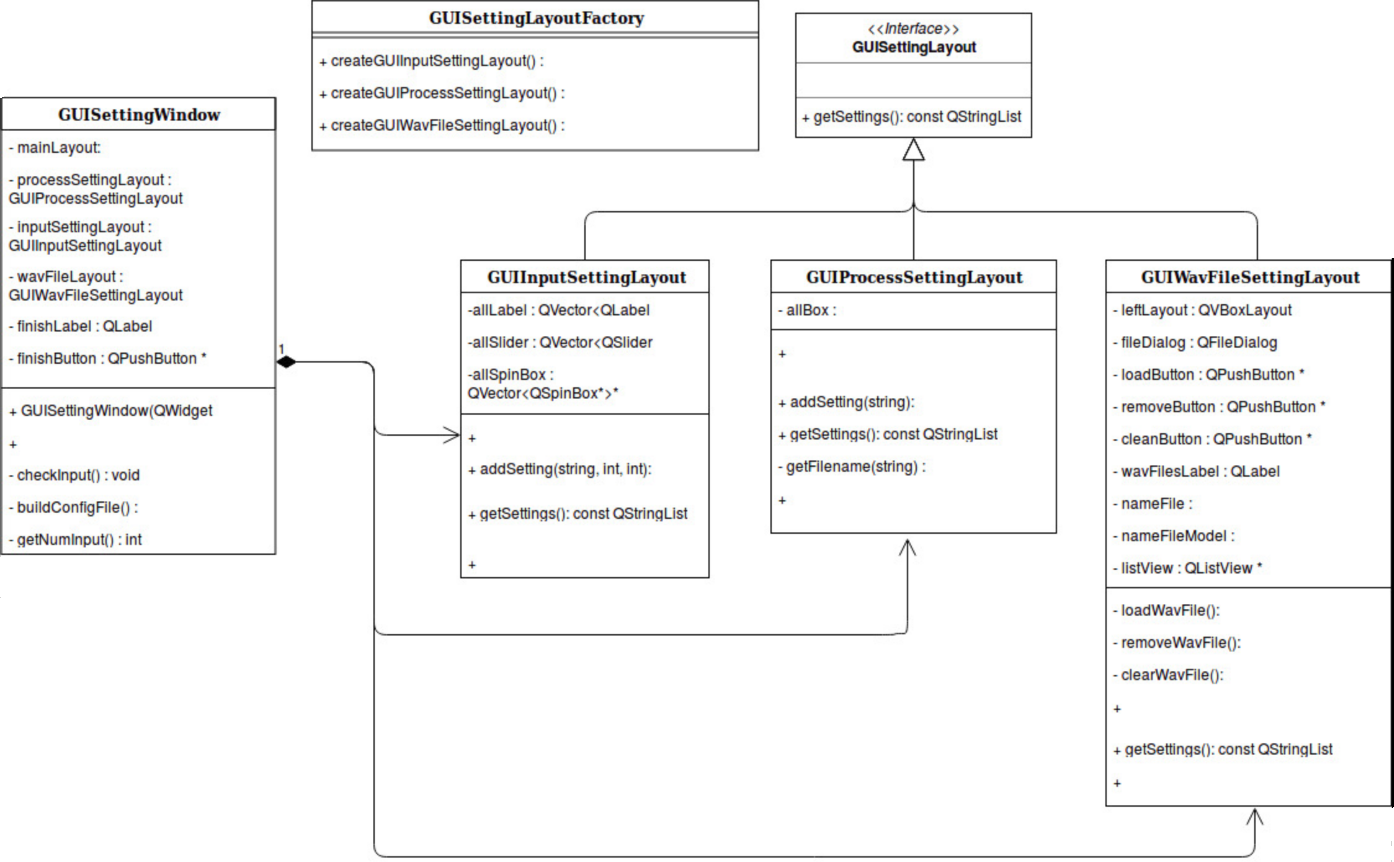
\includegraphics[scale=0.3]{umlSettingWindow.png}
 \verb!\caption{Schéma global du dispositif de VisualImpro}!
 \label{schéma global}
\end{figure}

\paragraph{}
La fenêtre de configuration

\begin{figure}[h]
 \centering
 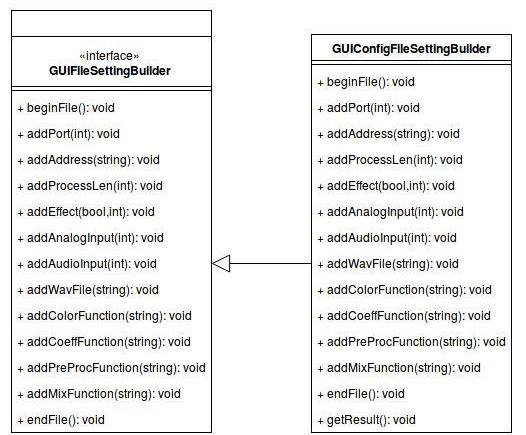
\includegraphics[scale=0.5]{umlBuilder.png}
 \verb!\caption{Schéma global du dispositif de VisualImpro}!
 \label{schéma global}
\end{figure}

\paragraph{}
La fenêtre de configuration

\subsection{Autres ajouts mineurs sur le programme}
